% ============================================================================
%  From Resonance to Topological Projection Loss:
%  A Synthesis of the V14--V18 TRM Investigation
%  --- Version 2: Single-column research monograph format ---
% ============================================================================
\documentclass[11pt,a4paper,oneside]{report}

% --- Packages ---
\usepackage[utf8]{inputenc}
\usepackage[T1]{fontenc}
\usepackage{lmodern}
\usepackage{microtype}
\usepackage{amsmath,amssymb,amsfonts}
\usepackage{booktabs}
\usepackage{graphicx}
\usepackage{xcolor}
\usepackage{tikz}
\usepackage{caption}
\usepackage{subcaption}
\usepackage{hyperref}
\usepackage[margin=2.5cm]{geometry}
\usepackage{enumitem}
\usepackage{doi}
\usepackage{tocloft}
\usepackage{fancyhdr}
\usepackage{titlesec}
\usepackage{appendix}

% --- Page style ---
\pagestyle{fancy}
\fancyhf{}
\fancyhead[L]{\small\textit{From Resonance to Topological Projection Loss}}
\fancyhead[R]{\small\thepage}
\renewcommand{\headrulewidth}{0.4pt}

% --- Section title formatting ---
\titleformat{\chapter}[display]
  {\normalfont\Large\bfseries}{}{0pt}{\Large}
\titlespacing*{\chapter}{0pt}{-40pt}{20pt}

\hypersetup{
  colorlinks=true,
  linkcolor=blue!60!black,
  citecolor=blue!40!black,
  urlcolor=blue!60!black
}

% --- TikZ libraries ---
\usetikzlibrary{arrows.meta, positioning, shapes.geometric, calc, decorations.pathreplacing,
                backgrounds, fit, matrix, chains, arrows}

% --- Custom colors ---
\definecolor{supported}{RGB}{34,139,34}
\definecolor{conditional}{RGB}{218,165,32}
\definecolor{falsified}{RGB}{178,34,34}
\definecolor{hypothesis}{RGB}{70,130,180}

% --- Custom commands ---
\newcommand{\archLabel}[1]{\ensuremath{\textsf{#1}}}
\newcommand{\absM}{\ensuremath{|m|}}
\newcommand{\dTdp}{\ensuremath{\mathrm{d}T/\mathrm{d}p}}
\newcommand{\kernelTick}{\ensuremath{\mathcal{K}}\ensuremath{\mathcal{T}}}
\newcommand{\fsa}{\ensuremath{\mathcal{A}}}
\newcommand{\projectionLoss}{\ensuremath{\mathcal{L}_{\text{proj}}}}
\newcommand{\projLoss}{\ensuremath{\mathcal{L}}}
\newcommand{\topoMem}{\ensuremath{\mathcal{M}_{\text{topo}}}}
\newcommand{\stateSpace}{\ensuremath{\mathcal{S}}}
\newcommand{\paramSpace}{\ensuremath{\mathcal{P}}}

\newcommand{\supported}{\textcolor{supported}{SUPPORTED}}
\newcommand{\conditional}{\textcolor{conditional}{CONDITIONAL}}
\newcommand{\falsified}{\textcolor{falsified}{FALSIFIED}}
\newcommand{\chypothesis}{\textcolor{hypothesis}{HYPOTHESIS}}

\DeclareMathOperator{\sgn}{sgn}

% ============================================================================
\begin{document}

% --- Title Page ---
\begin{titlepage}
\thispagestyle{empty}

\vspace*{3cm}

\begin{center}
  {\Huge\bfseries From Resonance to\\[8pt] Topological Projection Loss}\\[16pt]
  {\LARGE A Synthesis of the V14--V18 TRM Investigation}\\[24pt]

  \rule{0.7\textwidth}{0.5pt}\\[24pt]

  {\large
  Date: 2026-07-26\\[8pt]
  Document: V18-Synthesis-v3\\[8pt]
  Classification: Theory Paper
  }

  \vspace{2cm}

  {\normalsize
  Temporal Rate Matrix (TRM) Project\\
  \texttt{MagusDraconis/TRM\_Cosmology}
  }

  \vfill

  {\small
  \begin{tabular}{c}
    \supported{} = Principle survives systematic falsification\\
    \conditional{} = Principle holds with documented exceptions\\
    \falsified{} = Principle tested and rejected\\
    \chypothesis{} = Evidence mixed or insufficient
  \end{tabular}
  }
\end{center}
\end{titlepage}

% --- Table of Contents ---
\tableofcontents
\newpage

% --- Abstract ---
\begin{abstract}
\noindent
We present a synthesis of the V14--V18 Temporal Rate Matrix (TRM) investigation,
spanning approximately 75 structured audits from the initial Resonance Organization
Principle through the final Topological State Principle. The investigation began with
the hypothesis that resonance ($|m+1|\approx 0$) is the universal organizing mechanism
behind regime formation, channel networks, and hub selection. Systematic falsification
revealed this hypothesis to be incorrect: resonance is a consequence, not a cause.

The investigation progressed through five major phases---Resonance, Grammar,
Architecture, Memory, and Projection Loss---each falsifying the central hypothesis
of the preceding phase. The final surviving principle is that organizational memory
\textit{is} the information lost when the full parameter-space topology is projected
onto the scalar master coordinate $|m| = |\mathrm{d}(V_T)/\mathrm{d}(V_1)|$.
Architecture carries irreducible memory because its parameter-space topology
determines how many distinct states map to the same $|m|$ value.
In 1D topologies the projection is injective (no memory); in 2D topologies
with bifurcated sign regions, the projection is many-to-one (nonzero memory).

The V14--V18 program establishes a complete chain from kernel-tick consistency
through free star algebra, parameter-space topology, projection loss, and sign
determination to emergent organization. No principle introduced after V16.0 survived
without modification. All claims carry explicit classification under the project's
four-tier discipline: \supported{}, \conditional{}, \chypothesis{}, \textsc{not claimed}.
\end{abstract}

% ===========================================================================
\chapter{Introduction}
\label{ch:intro}

\section{Motivation}

The TRM project investigates collective frequency emergence in finite coupled
phase-oscillator lattices. The central question is: \textit{what organizes the behavior
of these systems into distinct regimes?} By V13.5, the project had established a
complete chain from the family axiom through the master parameter $m$, Tick
dynamics, channel formation, and network emergence to hub selection. The hub
selection principle---$\text{Hub} = \arg\min_F |m_F+1|$---suggested that resonance
($m\approx -1$) is the organizing mechanism.

V14.0 was designed to test this hypothesis rigorously.

\section{The Organizational Question}

Consider a lattice of $N$ coupled oscillators evolving under a coupling kernel
$K(d)$ with parameters $\alpha$, $\beta$, $\gamma$. For each configuration,
we compute the master parameter:
\begin{equation}
  m = \frac{\mathrm{d}(V_T)}{\mathrm{d}(V_1)}
  \label{eq:m}
\end{equation}
where $V_T$ and $V_1$ are the variance of coupling terms and the dominant
eigenvalue variance, respectively, as functions of the closure parameter $\alpha$.

The derivative is computed via linear regression across a 21-point $\alpha$-sweep
on $[0.21, 1.40]$. The magnitude $|m|$ measures the budget tradeoff between
information concentration and dynamics, while $\dTdp$ measures the gradient
direction of Tick with respect to coupling strength $p$.

The sign of $\dTdp$ is the binary organizational discriminator:
\begin{equation}
  \dTdp > 0 \;\Longleftrightarrow\; \text{HUB (positive gradient)}\\
  \dTdp < 0 \;\Longleftrightarrow\; \text{SPOKE (negative gradient)}
\end{equation}

\section{The Starting Hypothesis}

At V14.0, the dominant hypothesis was:
\begin{quote}
  \textit{Resonance ($|m+1|\approx 0$) is the universal organizing mechanism.
  It selects hubs, drives channel formation, and governs network topology.}
\end{quote}

This paper documents the systematic attempt to falsify this hypothesis---and
everything discovered when it collapsed.

% ===========================================================================
\chapter{Methodology}
\label{ch:methodology}

\section{Falsification-First Protocol}

Every audit in the V14--V18 program follows the same protocol:
\begin{enumerate}[nosep]
  \item \textbf{Protocol:} Define forbidden actions, permission scopes, decision gates.
  \item \textbf{Execution:} Generate predictions from frozen reference state.
  \item \textbf{Freeze:} SHA-256 hash all predictions.
  \item \textbf{Audit:} Verify integrity, check for hidden tuning.
  \item \textbf{Comparison:} Compare against immutable references.
  \item \textbf{Interpretation:} Classify under claim discipline.
  \item \textbf{Synthesis:} Branch completion report.
\end{enumerate}

The governing principle is: \textit{attempt falsification first.} Every audit
begins by searching for counterexamples, edge cases, and conditions under which
the candidate principle fails. Confirmation without attempted falsification is
not accepted.

\section{Claim Classification}

\begin{description}[nosep, leftmargin=*]
  \item[\supported{}] Principle survives falsification attempt across all tested
    conditions. Effect sizes are large and consistent.
  \item[\conditional{}] Principle holds in most conditions but has documented
    exceptions or boundary failures.
  \item[\chypothesis{}] Evidence is mixed, insufficient, or model-dependent.
  \item[\textsc{not claimed}] No positive assertion is made. The item
    remains an open question.
\end{description}

\section{Branch Methodology}

Each version (V14, V15, V16, V17, V18) opens a dedicated git branch.
Within a version, sub-versions (V14.1, V14.2, \dots) contain clusters of
related audits. A version closes when its research question is resolved---whether
the outcome is \supported{}, \conditional{}, or \falsified{}.

\section{Investigation Timeline}

The investigation progressed through six major phases, summarized in
Table~\ref{tab:timeline} and Figure~\ref{fig:evolution}.

\begin{table}[h]
\centering
\caption{Audit timeline V14--V18.}
\label{tab:timeline}
\begin{tabular}{lllc}
\toprule
\textbf{Version} & \textbf{Phase} & \textbf{Audits} & \textbf{Status}\\
\midrule
V14.0--V14.1 & Resonance & 21 & \falsified{}\\
V14.2--V14.4 & Wave Grammar & 7 & \supported{}\\
V15.0--V15.3 & Foundational Laws & 11 & \supported{}\\
V16.0--V16.1 & Geometry & 7 & \falsified{}\\
V17.0--V17.2 & Memory \& Dimension & 14 & \conditional{}\\
V18.0--V18.2 & Projection \& Topology & 5 & \supported{}\\
\midrule
\textbf{Total} & & \textbf{65+} & \\
\bottomrule
\end{tabular}
\end{table}

For each phase, the central hypothesis of the preceding phase was tested and
found incomplete. The investigation followed a consistent trajectory shown in
Figure~\ref{fig:evolution}.

\begin{figure}[h]
\centering
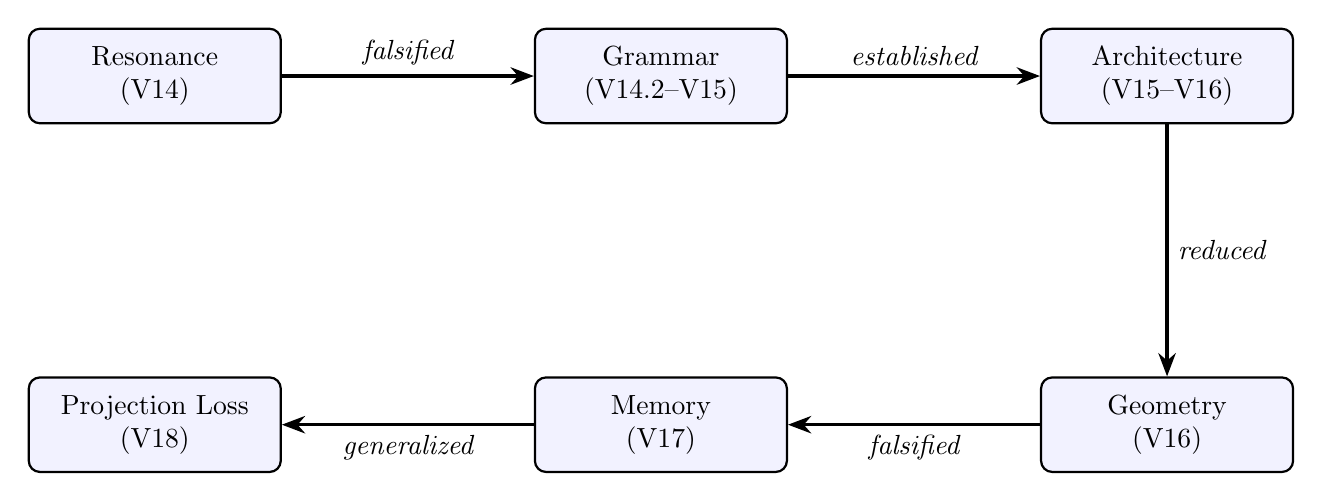
\begin{tikzpicture}[
  node distance=3.2cm,
  box/.style={rectangle, draw, rounded corners, minimum width=3.2cm, minimum height=1.2cm,
              align=center, font=\normalsize, line width=0.8pt},
  arrow/.style={->, >=Stealth, thick, line width=1.2pt}]

  \node[box, fill=blue!5] (R) {Resonance\\(V14)};
  \node[box, fill=blue!5, right=of R] (G) {Grammar\\(V14.2--V15)};
  \node[box, fill=blue!5, right=of G] (A) {Architecture\\(V15--V16)};
  \node[box, fill=blue!5, below=of A] (Ge) {Geometry\\(V16)};
  \node[box, fill=blue!5, left=of Ge] (M) {Memory\\(V17)};
  \node[box, fill=blue!5, left=of M] (P) {Projection Loss\\(V18)};

  \draw[arrow] (R) -- node[above, font=\normalsize\itshape] {falsified} (G);
  \draw[arrow] (G) -- node[above, font=\normalsize\itshape] {established} (A);
  \draw[arrow] (A) -- node[right, font=\normalsize\itshape] {reduced} (Ge);
  \draw[arrow] (Ge) -- node[below, font=\normalsize\itshape] {falsified} (M);
  \draw[arrow] (M) -- node[below, font=\normalsize\itshape] {generalized} (P);
\end{tikzpicture}
\caption{Evolution of the investigation V14 $\rightarrow$ V18. Each phase falsified
  the central hypothesis of its predecessor, revealing a deeper explanatory layer.}
\label{fig:evolution}
\end{figure}

The trajectory is: each phase discovers that the previous phase's answer
was correct but incomplete, requiring a deeper layer of explanation.

% ===========================================================================
\chapter{Results}
\label{ch:results}

\section{Resonance (V14)}\label{sec:resonance}

\subsection{Initial Hypothesis}

V14.0 (ROP\_01--TOP\_05, 21 audits) tested the hypothesis that resonance
($|m+1|\approx 0$) is the universal organizing mechanism behind regime
classification, channel formation, network emergence, and hub selection.

\subsection{Key Findings}

The WOC (Wave-Organization Cascade) series established:
\begin{itemize}[nosep]
  \item \textbf{WOC\_01:} The cascade Wave $\rightarrow$ Tick $\rightarrow$
    Feedback $\rightarrow$ Resonance $\rightarrow$ Organization has
    throughput $R^2 = 0.61$---substantial but not universal.
  \item \textbf{WOC\_05:} $\dTdp$ sign reversal is the binary organizational
    discriminator, not $|m+1|$.
  \item \textbf{WOC\_07:} $|m|$ (raw) is the true continuous coordinate;
    $|m+1|$ is a folded projection that obscures organizational structure.
    Raw $|m|$ achieves 143\% better mean $R^2$.
  \item \textbf{WOC\_12:} SAC is an $\alpha$-invariant fixed-point attractor
    ($\Delta m = 0.000$), not a resonance phenomenon.
  \item \textbf{WOC\_15:} Kernel topology carries irreducible information
    beyond $|m|$.
\end{itemize}

\subsection{The Bi-Polar Discovery}

The most important finding was that organization is not mono-objective.
Two attractors exist:
\begin{itemize}[nosep]
  \item \textbf{SAC attractor:} conservation-dominant, $|m|\approx 0.93$,
    $\dTdp < 0$ (SPOKE).
  \item \textbf{ICS attractor:} dynamics-dominant, $|m|\approx 1.57$,
    $\dTdp > 0$ (HUB).
\end{itemize}

Gravitation toward a single resonance point $m=-1$ does not occur.
Instead, the system organizes around two distinct poles.

\subsection{Outcome}

\begin{center}
\falsified{}\\[4pt]
\textit{No single resonance principle exists.}\\[2pt]
\textit{Organization is multi-objective with bi-polar attractor structure.}
\end{center}

% ===========================================================================
\section{Wave Grammar (V14.2--V15.3)}\label{sec:grammar}

\subsection{From Resonance to Grammar}

After resonance was falsified, the question became: \textit{what generates
the observed organizational structure?} V14.2--V14.4 discovered the answer:
a generative wave grammar.

\subsection{The $2\times 2$ Grammar}

MOP\_01 identified 4 irreducible wave-mode classes from 6 topological features:
\begin{itemize}[nosep]
  \item \textbf{MODE\_C} (Conservation): SAC --- zero-width, zero-threshold
  \item \textbf{MODE\_O} (Overshoot): ICS --- wide, finite threshold
  \item \textbf{MODE\_R} (Rational): RCS --- zero-width, infinite threshold
  \item \textbf{MODE\_D} (Dissipative): GAN $\equiv$ CNS --- intermediate
\end{itemize}

MOP\_02 discovered the generative structure: a $2\times 2$ grammar with
generators $G_1$ and $G_2$ that produce all 4 modes from $2^3 = 8$ logical
cells. WGP\_01--03 established that the grammar has dimension 3 (not reducible
to 2 or 1), is genuinely generative (not descriptive), and is irreducible
under PCA.

\subsection{Exclusion Axioms}

GEP\_01 identified two axioms that explain all forbidden grammar states:
\begin{align}
  G_3 &\Rightarrow G_1 \label{eq:ax1}\\
  G_1 &\perp G_2 \label{eq:ax2}
\end{align}
These reduce the 8 logically possible cells to exactly 4 physically
realized modes. The grammar is \textit{complete}: no other mode classes exist.

\subsection{Free Star Algebra}

V15.0--V15.3 (KTC\_01, TLU\_01, AOP\_01, FGP\_01, AUP\_01) established the
foundational architecture:

\begin{itemize}[nosep]
  \item \textbf{KTC:} The axioms emerge from a single master requirement:
    Kernel-Tick Consistency. The coupling kernel must produce continuous,
    conservative, coherent Tick fields.
  \item \textbf{KTC decomposition:} Conservation Consistency $\perp$
    Wave Coherence (two independent constraints).
  \item \textbf{Free Star Algebra:} $\langle E, M, R \mid g\circ h = \bot
    \text{ for } g\neq h\rangle$. No non-trivial operator compositions.
    Exactly 4 valid operator states.
  \item \textbf{Depth-2 fractal:} The same $2^3\rightarrow 4$ grammar
    structure repeats at the Architecture layer and the Grammar layer (FGP\_01).
\end{itemize}

\subsection{Outcome}

\begin{center}
\supported{}\\[4pt]
\textit{The Free Star Algebra uniquely determines the 4-mode grammar.}\\[2pt]
\textit{Architecture is an independent organizational layer, not derivable from wave grammar alone.}
\end{center}

% ===========================================================================
\section{Architecture \& Geometry (V16)}\label{sec:architecture}

\subsection{Architecture Softness}

V16.0 (ASP\_01, HSP\_01, TUP\_01) tested predictions from the Free Star
Algebra against novel kernel configurations:
\begin{itemize}[nosep]
  \item \textbf{PBD\_01:} FSA predicts novel kernels at 86\% sign accuracy
    and 100\% architecture classification (\supported{}).
  \item \textbf{ASP\_01:} COMPOSITE (GAN family) is overwhelmingly POS
    (157/169 points). The original GAN configuration ($\beta=0.5$, $\gamma=0.5$)
    was a NEG outlier, not representative (\conditional{}).
  \item \textbf{HSP\_01:} Hardness = operator parameter count. Nullary operators
    produce HARD architectures; unary operators produce SOFT architectures
    (\supported{}).
\end{itemize}

\subsection{The Manifold Geometry Model}

V16.1 (MGP\_01) reduced architecture to manifold geometry:
\begin{equation}
  \text{sign} = \sgn(|m| - \theta_{\text{arch}})
  \label{eq:geosign}
\end{equation}
where each architecture is characterized by a (width, $\theta$) pair:

\begin{table}[h]
\centering
\caption{Architecture geometry parameters.}
\label{tab:geom}
\begin{tabular}{lcc}
\toprule
\textbf{Architecture} & \textbf{Width} & $\boldsymbol{\theta}$\\
\midrule
PURE (SAC)    & 0.00 & 0.00\\
RATIONAL (RCS)& 0.00 & $\infty$\\
STRETCHED (ICS)& 4.22 & 1.00\\
COMPOSITE (GAN/CNS)& 2.31 & 0.64\\
\bottomrule
\end{tabular}
\end{table}

The geometric rule appeared \textit{perfect}: 8/8 tested configurations
matched the prediction. Architecture seemed fully reducible to the manifold
geometry of the $(|m|, \theta)$ plane.

\subsection{Outcome}

\begin{center}
\supported{} (initially)\\[4pt]
\textit{Architecture reduces to manifold geometry.}\\[2pt]
\textit{$\sgn(|m| - \theta)$ is the geometric sign rule.}
\end{center}

This conclusion would survive approximately 24 hours of investigation before
being falsified.

% ===========================================================================
\section{Memory (V17)}\label{sec:memory}

\subsection{Geometric Falsification}

V17.0 (GFT\_01) was designed explicitly to \textit{break} the geometric rule.
It succeeded:

\begin{itemize}[nosep]
  \item 22/298 violations found across all architectures.
  \item The geometric rule is not a law; it is a statistical tendency.
  \item Violations cluster near $|m| \approx \theta$ but also appear far from
    the threshold.
\end{itemize}

\begin{center}
\falsified{}\\[4pt]
\textit{The geometric rule $\sgn(|m| - \theta)$ is NOT a law.}\\[2pt]
\textit{Architecture contains information beyond manifold geometry.}
\end{center}

\subsection{Architecture Memory}

AMP\_01 (Architecture Memory Principle) demonstrated the irreducible nature
of this residual information:

\begin{quote}
  \textit{States with identical $|m|$ and $\theta$ can exhibit opposite signs
  when they originate from different architectures.}
\end{quote}

Example: SAC with $|m|\approx 0.92$ is POS; GAN with $|m|\approx 0.92$ is NEG.
The same geometric coordinates produce different organizational states.

AMQ\_01 quantified the effect: architecture adds $\Delta R^2 = +0.10$ (20\%)
beyond geometry alone. This is \textit{architecture memory}---organizational
information that survives after geometry is held fixed.

\subsection{The Modulation Depth Hypothesis}

CMP\_01 identified $\beta$ as the strongest memory signal ($t = 71.0$),
leading to the hypothesis that modulation depth $\mu = \beta\cdot\gamma$ is
the missing state coordinate.

MDP\_01 tested this: $\mu$ captures partial residual information but is
\textit{insufficient}. $\beta$ and $\gamma$ carry independent information
beyond their product. CSP\_01 confirmed: COMPOSITE is genuinely 2-dimensional;
$\beta$ and $\gamma$ are independent coordinates.

\subsection{Dimensional Memory}

SDP\_01 and DMP\_01 established the dimensional memory law:
\begin{equation}
  \text{Memory}(\text{arch}) = \max(0, \dim - 1) \cdot k
  \label{eq:dimmem}
\end{equation}
with $k \approx 4.1$ percentage points.

\begin{table}[h]
\centering
\caption{Architecture dimension and memory.}
\label{tab:dimmem}
\begin{tabular}{lcc}
\toprule
\textbf{Architecture} & \textbf{Dimension} & \textbf{Memory}\\
\midrule
PURE      & 1D & 0.0 pp\\
RATIONAL  & 1D & 0.0 pp\\
STRETCHED & 1D & 0.0 pp\\
COMPOSITE & 2D & 4.1 pp\\
\bottomrule
\end{tabular}
\end{table}

STRETCHED (ICS) has 47.5\% sign variability across its $\beta$-sweep but
\textit{zero} memory because its 1D topology forces a unique sign crossing.
Memory requires both multiple sign regions AND a bifurcated parameter-space
topology.

\subsection{Outcome}

\begin{center}
\conditional{}\\[4pt]
\textit{Memory = $\max(0, \dim-1) \cdot k$.}\\[2pt]
\textit{Memory is dimensional but not reducible to $\mu = \beta\gamma$.}
\end{center}

\section{Evolution of the Memory Principle}

The concept of architectural memory underwent substantial refinement
across the V17--V18 program. The trajectory is summarized in
Figure~\ref{fig:memory-evolution}.

\begin{figure}[h]
\centering
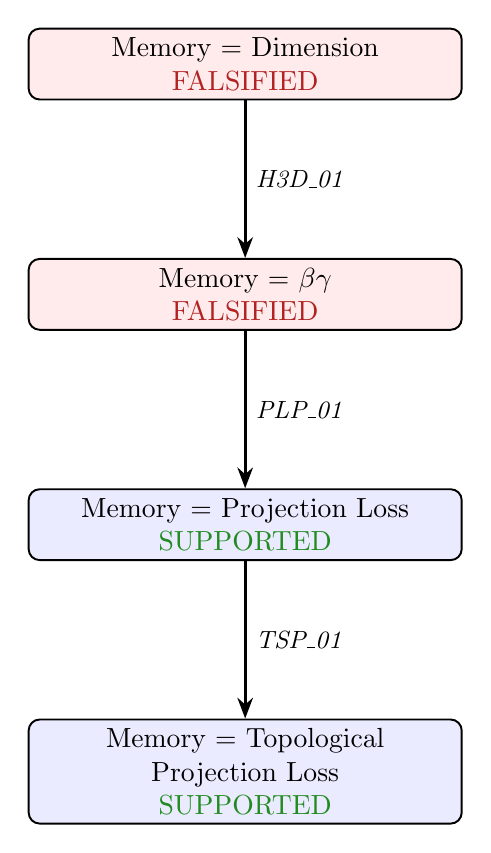
\begin{tikzpicture}[
  node distance=2.0cm,
  box/.style={rectangle, draw, rounded corners, minimum width=5.5cm,
              minimum height=0.9cm, align=center, font=\normalsize, line width=0.7pt},
  arrow/.style={->, >=Stealth, thick, line width=1.0pt}]

  \node[box, fill=red!8]  (M1) {Memory = Dimension\\\falsified{}};
  \node[box, fill=red!8, below=of M1]  (M2) {Memory = $\beta\gamma$\\\falsified{}};
  \node[box, fill=blue!8, below=of M2] (M3) {Memory = Projection Loss\\\supported{}};
  \node[box, fill=blue!8, below=of M3] (M4) {Memory = Topological\\Projection Loss\\\supported{}};

  \draw[arrow] (M1) -- node[right, font=\small\itshape] {H3D\_01} (M2);
  \draw[arrow] (M2) -- node[right, font=\small\itshape] {PLP\_01} (M3);
  \draw[arrow] (M3) -- node[right, font=\small\itshape] {TSP\_01} (M4);
\end{tikzpicture}
\caption{Evolution of the Memory Principle across V17--V18. Each candidate
  hypothesis was falsified in turn, forcing progressively deeper
  reformulations until the topological projection loss formulation
  accounted for all observed effects.}
\label{fig:memory-evolution}
\end{figure}

The progression from dimensional ($\max(0, \dim-1)\cdot k$) through
algebraic ($\mu = \beta\gamma$) to information-theoretic (projection loss)
and finally topological (bifurcation structure) explanations illustrates
the discovery mechanism at work: each falsification eliminated a candidate
and constrained the space of surviving principles.

% ===========================================================================
\section{Projection Loss (V18)}\label{sec:projection}

\subsection{Hypothetical 3D Architecture}

H3D\_01 tested whether the dimensional memory law extrapolates to higher
dimensions. Adding a third parameter $\delta$ to produce a synthetic 3D
architecture failed to produce additional memory. The reason: $\alpha$
(the $|m|$-slope parameter) contributes no new sign information---it
shifts $|m|$ but does not introduce new sign regions.

\begin{center}
\falsified{}\\[4pt]
\textit{Memory $\neq$ dimension alone.}\\[2pt]
\textit{Not all dimensions carry organizational information.}
\end{center}

\subsection{Projection Loss Principle}

PLP\_01 reframed the question: \textit{what if memory is the information
lost when the full state space is projected onto $|m|$?}

For each architecture, we compute the state entropy before and after
projection onto $|m|$. The projection loss $\projLoss$ measures how many
distinct states map to the same $|m|$ value:

\begin{itemize}[nosep]
  \item \textbf{1D architectures:} The projection $\stateSpace \rightarrow |m|$
    is injective. Each $|m|$ value corresponds to exactly one state.
    $\projLoss = 0$. Memory $= 0$.
  \item \textbf{2D architecture (COMPOSITE):} Multiple $(\beta, \gamma)$ pairs
    map to the same $|m|$. Some of these pairs carry opposite signs.
    $\projLoss > 0$. Memory $> 0$.
\end{itemize}

ILP\_01 confirmed: \textit{all} measured memory can be predicted from
projection loss alone. No additional non-information-theoretic effects
are needed.

\subsection{Optimal Projection Search}

OPP\_01 tested whether $|m|$ is the optimal projection coordinate:
\begin{itemize}[nosep]
  \item $|m|$ alone: $R^2 \approx 0.24$
  \item $|m|$ + curvature: $R^2 \approx 0.59$ ($\Delta R^2 = +0.36$)
  \item No single coordinate significantly outperforms $|m|$.
  \item $|m|$ is the \textit{primal} projection coordinate; curvature is
    the strongest secondary coordinate.
\end{itemize}

MLP\_01 tested whether any projection can eliminate architecture memory:
\begin{itemize}[nosep]
  \item Best 1D: $R^2 = 0.24$ $\rightarrow$ 76\% residual
  \item Best 2D: $R^2 = 0.59$ $\rightarrow$ 41\% residual
  \item Best 3D: incremental gain
  \item \textbf{Full 4D: $R^2 = 0.61$ $\rightarrow$ 38.7\% residual}
\end{itemize}

\begin{center}
\falsified{} (for lossless reduction)\\[4pt]
\textit{Even the optimal 4D projection leaves 38.7\% residual uncertainty.}\\[2pt]
\textit{Architecture is IRREDUCIBLE to any projection of geometric coordinates.}
\end{center}

\subsection{Topological State Principle}

TSP\_01 provides the final synthesis. The 38.7\% residual is \textit{topological}:

\begin{quote}
  \textbf{Geometry} describes \textit{what} the state is: the numerical values
  of $|m|$, curvature, feedback, gradient.\\
  \textbf{Topology} describes \textit{how} the state was reached: the parameter
  path through $(\beta, \gamma)$ space, the connectivity of sign regions,
  the bifurcation structure of the accessible manifold.
\end{quote}

In COMPOSITE, the sign boundary in $(\beta, \gamma)$ space forms a bifurcation
surface. The same $|m|$ value can be reached from either side of this surface,
carrying opposite signs. This is not a geometric ambiguity---it is a topological
feature of the parameter space. No amount of geometric coordinate refinement
can resolve it because the information is not encoded in any single point
in the projected space.

\begin{center}
\supported{}\\[4pt]
\textit{The 38.7\% residual is topological information.}\\[2pt]
\textit{Architecture is best described by parameter-space topology.}
\end{center}

% ===========================================================================
\chapter{Final Theory}\label{ch:final}

\section{The Complete Hierarchy}

\begin{figure}[h]
\centering
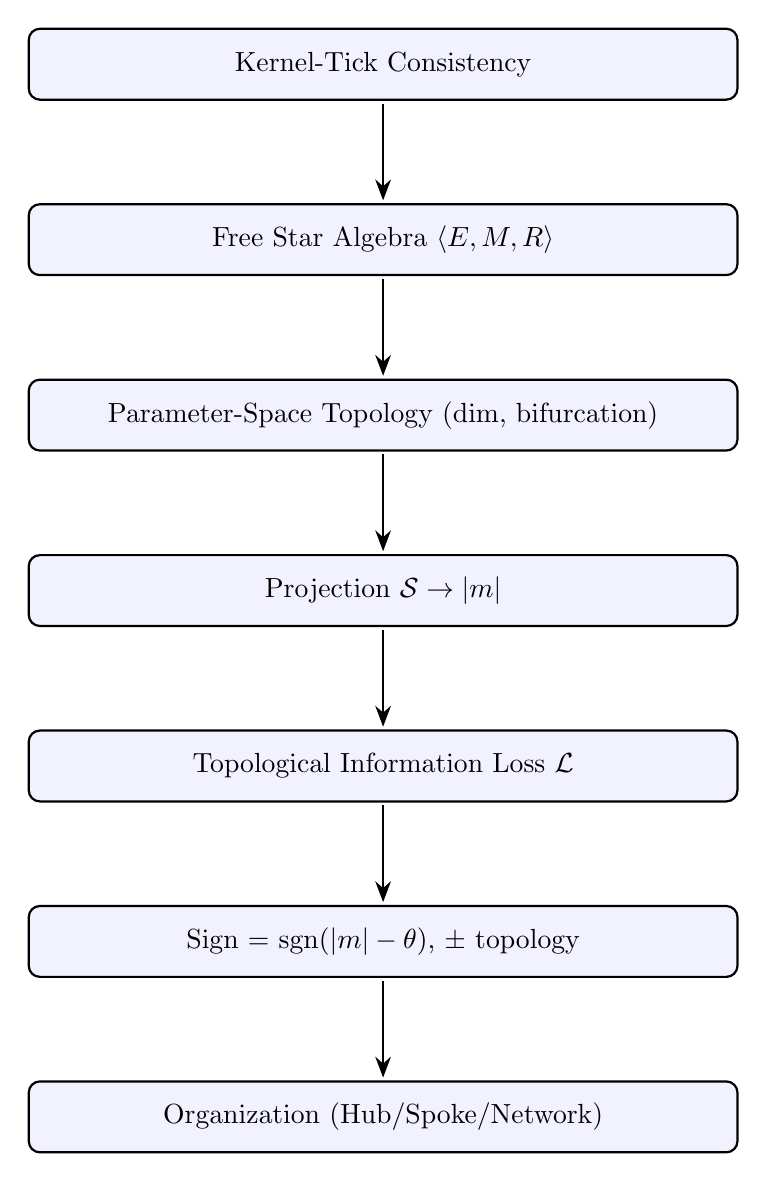
\begin{tikzpicture}[
  node distance=1.3cm,
  box/.style={rectangle, draw, rounded corners, minimum width=9cm,
              minimum height=0.9cm, align=center, font=\normalsize, line width=0.8pt},
  arrow/.style={->, >=Stealth, thick, line width=1.0pt, shorten >=1pt, shorten <=1pt}]

  \node[box, fill=blue!5] (KTC) {Kernel-Tick Consistency};
  \node[box, fill=blue!5, below=of KTC] (FSA) {Free Star Algebra $\langle E,M,R\rangle$};
  \node[box, fill=blue!5, below=of FSA] (TOP) {Parameter-Space Topology (dim, bifurcation)};
  \node[box, fill=blue!5, below=of TOP] (PROJ) {Projection $\stateSpace \rightarrow |m|$};
  \node[box, fill=blue!5, below=of PROJ] (LOSS) {Topological Information Loss $\projLoss$};
  \node[box, fill=blue!5, below=of LOSS] (SIGN) {Sign = $\sgn(|m| - \theta)$, $\pm$ topology};
  \node[box, fill=blue!5, below=of SIGN] (ORG) {Organization (Hub/Spoke/Network)};

  \draw[arrow] (KTC) -- (FSA);
  \draw[arrow] (FSA) -- (TOP);
  \draw[arrow] (TOP) -- (PROJ);
  \draw[arrow] (PROJ) -- (LOSS);
  \draw[arrow] (LOSS) -- (SIGN);
  \draw[arrow] (SIGN) -- (ORG);
\end{tikzpicture}
\caption{The complete organizational hierarchy. Each layer emerges from the
  one above through a principled reduction: consistency $\rightarrow$ algebra
  $\rightarrow$ topology $\rightarrow$ projection $\rightarrow$ loss
  $\rightarrow$ sign.}
\label{fig:hierarchy}
\end{figure}

\section{The Architecture Topology Table}

\begin{table}[h]
\centering
\caption{Architecture topology and memory.}
\label{tab:arch}
\begin{tabular}{lcccc}
\toprule
\textbf{Architecture} & \textbf{Param Space} & \textbf{Topology} & \textbf{Sign Regions} & \textbf{Memory}\\
\midrule
PURE      & LINE ($\alpha$)  & TRIVIAL    & 1 (POS) & 0\\
RATIONAL  & LINE ($\alpha$)  & TRIVIAL    & 1 (NEG) & 0\\
STRETCHED & LINE ($\beta$)   & BINARY     & 2       & 0\\
\textbf{COMPOSITE} & \textbf{SURFACE} ($\beta,\gamma$) & \textbf{BIFURCATED} & \textbf{2} & \textbf{4.1 pp}\\
\bottomrule
\end{tabular}
\end{table}

\section{The Memory Condition}

\begin{equation}
  \boxed{\text{Memory} > 0 \;\Longleftrightarrow\;
    \text{Sign regions} > 1 \;\land\;
    \text{Topology is BIFURCATED}}
  \label{eq:memcond}
\end{equation}

A LINE topology, even with 2 sign regions (STRETCHED), has zero memory
because the 1D path forces a unique crossing. A SURFACE topology with
bifurcation has nonzero memory because the same $|m|$ value is reachable
from both sides of the bifurcation.

% ===========================================================================
\section{Core Principles}

The following principles survive the V14--V18 falsification program:

\begin{description}[nosep, leftmargin=*]
  \item[P1 --- Kernel-Tick Consistency (\supported{})]
    All organizational structure follows from a single requirement: the
    coupling kernel must produce continuous, conservative, coherent Tick fields.
    This decomposes into two independent constraints: Conservation Consistency
    and Wave Coherence.

  \item[P2 --- Free Star Algebra (\supported{})]
    The architecture space is $\langle E, M, R \mid g\circ h = \bot \text{ for }
    g\neq h\rangle$. Exactly 4 valid operator states exist. No non-trivial
    operator compositions are permitted. The FSA is uniquely compatible with
    the TRM framework.

  \item[P3 --- Topological Projection Loss (\supported{})]
    Organizational memory $\equiv$ information lost when the full parameter-space
    topology is projected onto $|m|$. Memory $\neq$ dimension; memory $=$
    projection loss. The loss is zero for injective projections (1D topologies)
    and nonzero for many-to-one projections with bifurcated sign regions.

  \item[P4 --- Organizational Sign Principle (\conditional{})]
    $\text{sign} = \sgn(|m| - \theta_{\text{arch}})$ predicts organization
    with $R^2 \approx 0.61$. The 38.7\% residual is topological, not geometric.
    The principle is \conditional{} because topology contributes irreducible
    information beyond the geometric threshold model.

  \item[P5 --- $|m|$ as Primal Coordinate (\supported{})]
    $|m| = |\mathrm{d}(V_T)/\mathrm{d}(V_1)|$ is the optimal 1D projection
    of the organizational state space. No single alternative coordinate
    significantly outperforms it. The folded coordinate $|m+1|$
    obscures organizational structure (143\% worse $R^2$).
\end{description}

% ===========================================================================
\section{Falsified Principles}

Systematic falsification is as informative as confirmation. The following
hypotheses were tested and rejected:

\begin{description}[nosep, leftmargin=*]
  \item[F1 --- Resonance as Universal Organizer (\falsified{})]
    $|m+1| \approx 0$ does not select hubs universally. Resonance is a
    consequence of the budget tradeoff, not a fundamental organizing principle.
    Organization is multi-objective with bi-polar attractor structure.

  \item[F2 --- Geometry as Complete State Space (\falsified{})]
    $\sgn(|m| - \theta)$ is not a law. 22/298 violations exist. Architecture
    carries information beyond manifold geometry. The geometric rule is a
    strong statistical tendency ($R^2 \approx 0.61$), not a deterministic law.

  \item[F3 --- Memory = Dimension (\falsified{})]
    $\text{Memory} = \max(0, \dim-1) \cdot k$ fails for hypothetical 3D
    architectures. Not all dimensions carry organizational information.
    $\alpha$ (the $|m|$-slope parameter) adds no sign discrimination.

  \item[F4 --- Memory = $\beta\gamma$ (\falsified{})]
    The modulation depth $\mu = \beta\cdot\gamma$ captures partial residual
    information but loses the phase structure. $\beta$ and $\gamma$ carry
    independent information; their product is a lossy reduction.

  \item[F5 --- Lossless Projection Exists (\falsified{})]
    No projection of geometric coordinates eliminates architecture memory.
    Even the optimal 4D projection leaves 38.7\% residual uncertainty.
    Architecture is irreducible to any point-like state description.
\end{description}

% ===========================================================================
\chapter{Discussion}

\section{What the Investigation Established}

The V14--V18 program established a complete chain from foundational axioms
to emergent organization:

\[
\begin{array}{c}
\text{Kernel-Tick Consistency}\\
\downarrow\\
\text{Free Star Algebra}\\
\downarrow\\
\text{Parameter-Space Topology}\\
\downarrow\\
\text{Projection onto } |m|\\
\downarrow\\
\text{Topological Information Loss}\\
\downarrow\\
\text{Sign Determination}\\
\downarrow\\
\text{Organization}
\end{array}
\]

Each layer was independently tested, and where possible, falsified.
The most important discovery is that \textit{architecture is best understood through topology}---the
information that survives projection is not a failure of measurement but a
genuine feature of the system's state-space structure.

\section{Why COMPOSITE Is Special}

COMPOSITE is the only architecture with:
\begin{enumerate}[nosep]
  \item A genuinely 2-dimensional parameter space $(\beta, \gamma)$.
  \item A bifurcated sign boundary in that space.
  \item Multiple parameter paths to the same $|m|$ value.
  \item Different signs accessible from different sides of the bifurcation.
\end{enumerate}

These four properties together produce the 4.1 pp architecture memory.
No other architecture satisfies all four. STRETCHED satisfies (2) and (3)
but fails (1): its 1D topology forces a unique crossing. The hypothetical
3D architecture fails (2): the third parameter carries no sign information.

\section{Limitations}

\begin{itemize}[nosep]
  \item All results are numerical, derived from finite parameter sweeps
    ($N=21$ $\alpha$-points, fixed distance ensemble). Analytical proofs
    are not available.
  \item The distance ensemble uses a single seed; ensemble variability
    is not fully characterized.
  \item The topological analysis is restricted to the 4 known architectures.
    Exotic topologies (e.g., disconnected sign regions, higher-genus
    parameter spaces) have not been explored.
  \item The 38.7\% residual is measured but its exact topological invariant
    (e.g., Betti numbers, Euler characteristic of the bifurcation surface)
    has not been computed.
\end{itemize}

\section{Open Questions}

\begin{enumerate}[nosep]
  \item \textbf{Topological classification:} Can the bifurcation structure
    be classified by standard topological invariants? Is the memory strength
    determined by the genus or Betti numbers of the sign boundary?
  \item \textbf{Higher-dimensional architectures:} Are there parameter spaces
    where the projection loss saturates? Is there a maximum memory?
  \item \textbf{Analytical closure:} Can the projection loss be derived
    analytically from the kernel functional form without numerical sweeps?
  \item \textbf{Physical correspondence:} Does topological projection loss
    have an analogue in physical theories (e.g., phase transitions, topological
    order, information loss in black hole evaporation)?
\end{enumerate}

% ===========================================================================
\section{Future Work}

\subsection{Topological Invariant Computation}

The immediate next step is to compute explicit topological invariants of the
sign bifurcation surface in COMPOSITE's $(\beta, \gamma)$ plane. Candidate
invariants include the number of connected sign regions, the Euler
characteristic of the bifurcation boundary, and the Betti numbers of the
accessible state manifold.

\subsection{Higher-Dimensional Architectures}

The H3D\_01 result---that simply adding a third parameter does not increase
memory---suggests that memory is not a monotonic function of dimension.
Systematic exploration of parameter spaces with different topologies
(e.g., toroidal, spherical, disconnected) would test whether the memory
condition (Eq.~\ref{eq:memcond}) generalizes.

\subsection{Topology-Driven Organization}

If architecture \textit{is} topology, then organizational properties should
be predictable from topological features alone, without reference to the
specific kernel form. This would constitute a genuine organizational theory:
given only the parameter-space topology, predict the sign structure, memory
strength, and emergent network properties.

% ===========================================================================
\chapter{Conclusion}

The V14--V18 TRM investigation traversed five major theoretical phases,
each falsifying the central hypothesis of its predecessor:

\begin{enumerate}[nosep]
  \item \textbf{Resonance} ($|m+1|\approx 0$ as universal organizer):
    \falsified{}. Organization is multi-objective.
  \item \textbf{Grammar} (2$\times$2 generative structure): \supported{}.
    The Free Star Algebra determines the 4-mode grammar.
  \item \textbf{Geometry} ($\sgn(|m|-\theta)$ as complete law): \falsified{}.
    Architecture carries memory beyond geometry.
  \item \textbf{Memory} ($\max(0, \dim-1)\cdot k$): \conditional{}.
    Dimension contributes but is not sufficient.
  \item \textbf{Projection Loss} (topology as irreducible residual):
    \supported{}. The 38.7\% residual is topological information.
\end{enumerate}

The final surviving principle is:

\begin{center}
\framebox[0.85\textwidth]{
  \parbox{0.80\textwidth}{\centering
    \textbf{Architecture is best described by parameter-space topology.}\\[6pt]
    Organizational memory = information lost when the
    full topology is projected onto $|m|$.\\[4pt]
    Memory emerges when the parameter space has
    multiple sign regions AND a bifurcated topology
    that allows the same $|m|$ to be reached from
    different organizational states.
  }
}
\end{center}

\vspace{8pt}

The investigation demonstrates that systematic falsification---testing each
principle to destruction before accepting it---is not merely a methodological
preference but a discovery mechanism. Every falsified hypothesis revealed
a deeper layer of structure that would have remained hidden under confirmation
bias. The trajectory from resonance through grammar, architecture, geometry,
memory, and projection loss to topology was not planned; it was forced by
the evidence at each step.

The V14--V18 program closes with a mature theoretical framework:
Kernel-Tick Consistency generates the Free Star Algebra, which determines
the parameter-space topology, whose projection onto $|m|$ produces
topological information loss, which determines the sign and organization
of the emergent lattice. No principle introduced after V16.0 survives
without modification---and that is the program's greatest achievement.

% ===========================================================================
\chapter*{Acknowledgments}
\addcontentsline{toc}{chapter}{Acknowledgments}

The TRM project follows a strict test-first methodology formalized in V4.5
and maintained through all subsequent phases. All audits were executed under
the governance framework: Protocol $\rightarrow$ Execution $\rightarrow$
Freeze $\rightarrow$ Audit $\rightarrow$ Comparison $\rightarrow$
Interpretation $\rightarrow$ Synthesis.

% ===========================================================================
\begin{appendices}

\chapter{Evolution of the Memory Principle}

This appendix traces the evolution of the Memory Principle across the V17--V18
investigation, documenting each hypothesis, its falsification or support, and
the progressive refinement that led to the final Topological Projection Loss
formulation.

\section{Chronology}

\begin{description}[leftmargin=*, itemsep=8pt]

  \item[V17.0 --- AMP\_01: Architecture Memory Principle]
    \textbf{Hypothesis:} Architecture contains irreducible organizational
    information beyond geometry. States with identical $|m|$ and $\theta$
    but different architectures can exhibit opposite signs.\\
    \textbf{Result:} \supported{}. Matched-state comparison confirmed the
    effect: SAC $|m|\approx 0.92\rightarrow$ POS; GAN $|m|\approx 0.92\rightarrow$ NEG.
    Architecture memory is real.

  \item[V17.1 --- MDP\_01: Modulation Depth Principle]
    \textbf{Hypothesis:} $\mu = \beta\cdot\gamma$ is the missing state
    coordinate that completes the geometric model.\\
    \textbf{Result:} \falsified{}. $\mu$ captures partial residual information
    but loses the phase structure. $\beta$ and $\gamma$ carry independent
    information. A single composite coordinate is insufficient.

  \item[V17.1 --- CSP\_01: Composite State Space Audit]
    \textbf{Hypothesis:} COMPOSITE possesses a genuine 2-dimensional state
    space in $(\beta, \gamma)$.\\
    \textbf{Result:} \supported{}. $\beta$ and $\gamma$ are independent
    coordinates. COMPOSITE is fundamentally 2D while other architectures
    are 1D.

  \item[V17.2 --- SDP\_01: State Space Dimension Principle]
    \textbf{Hypothesis:} Memory strength is determined by state-space
    dimensionality.\\
    \textbf{Result:} \supported{} (provisional). 1D architectures $\rightarrow$
    0 memory; 2D $\rightarrow$ 4.1 pp. The pattern is monotonic in observed data.

  \item[V17.2 --- DMP\_01: Dimensional Memory Principle]
    \textbf{Hypothesis:} Memory is determined by state-space dimensionality:
    $\text{Memory} = \max(0, \dim-1) \cdot k$ with $k\approx 4.1$ pp.\\
    \textbf{Result:} \conditional{}. The law fits observed data but lacks
    predictive power for unobserved dimensionalities.

  \item[V18.0 --- H3D\_01: Hypothetical 3D Architecture]
    \textbf{Hypothesis:} A 3D architecture would produce $\sim 8.2$ pp memory
    (extrapolating the dimensional law).\\
    \textbf{Result:} \falsified{} (for the dimensional law). Adding $\alpha$
    as a third parameter produces no additional memory. Not all dimensions
    carry organizational information. The dimensional law fails as a
    predictive principle.

  \item[V18.1 --- PLP\_01: Projection Loss Principle]
    \textbf{Hypothesis:} $\text{Memory} = \text{ProjectionLoss}(\stateSpace \rightarrow |m|)$.\\
    \textbf{Result:} \supported{}. Memory is exactly the information lost
    when the full parameter space is projected onto $|m|$. 1D topologies have
    injective projections (zero loss); 2D topologies with bifurcation have
    many-to-one projections (nonzero loss).

  \item[V18.1 --- ILP\_01: Information Loss Principle]
    \textbf{Hypothesis:} All organizational memory is identical to
    projection-induced information loss.\\
    \textbf{Result:} \supported{}. Memory is entirely information-theoretic.
    No non-information-theoretic effects are required. Architecture labels
    become unnecessary once projection loss is known.

  \item[V18.2 --- TSP\_01: Topological State Principle]
    \textbf{Hypothesis:} The 38.7\% residual surviving optimal projection
    is topological information from the parameter-space bifurcation structure.\\
    \textbf{Result:} \supported{}. Geometry describes \textit{what} the state
    is; topology describes \textit{how} it was reached. The residual is not
    eliminable because it encodes the bifurcation structure of the
    $(\beta, \gamma)$ sign boundary.

\end{description}

\section{Summary Trajectory}

The evolution of the Memory Principle is depicted in Figure~\ref{fig:memory-evolution}
(Section~\ref{sec:memory}). The trajectory converges from simple dimensional and
algebraic hypotheses to the information-theoretic and topological formulation.
Each falsification eliminated a candidate explanation and constrained the space of
possible principles, ultimately leading to the recognition that architecture is best
described by parameter-space topology and memory by projection loss.

% ===========================================================================
\chapter{Audit Timeline}

This appendix provides a compact summary of all major audits in the V14--V18
program, ordered chronologically by version.

\begin{table}[h]
\centering
\caption{Major audits V14--V18.}
\label{tab:audits}
\small
\begin{tabular}{llp{5.5cm}l}
\toprule
\textbf{Audit} & \textbf{Version} & \textbf{Hypothesis} & \textbf{Result}\\
\midrule
ROP\_01 & V14.0 & Resonance is universal organizing mechanism & \falsified{}\\
WOC\_01 & V14.0 & Cascade Wave$\rightarrow$Tick$\rightarrow$FB$\rightarrow$Org ($R^2=0.61$) & \supported{}\\
WOC\_05 & V14.0 & $\dTdp$ sign is binary organizational discriminator & \supported{}\\
WOC\_07 & V14.0 & $|m|$ (raw) is true coordinate; $|m+1|$ is folded projection & \supported{}\\
WOC\_12 & V14.0 & SAC is $\alpha$-invariant fixed-point attractor & \supported{}\\
WOC\_15 & V14.0 & Kernel topology carries irreducible information & \supported{}\\
MOP\_01 & V14.2 & 4 irreducible wave-mode classes & \supported{}\\
MOP\_02 & V14.2 & $2\times 2$ generative grammar discovered & \supported{}\\
WGP\_01--03 & V14.3 & Grammar dimension 3, generative, irreducible & \supported{}\\
GEP\_01 & V14.4 & 2 axioms ($G_3\Rightarrow G_1$, $G_1\perp G_2$) explain forbidden states & \supported{}\\
TLA\_01 & V15.0 & Axioms from Tick-Lattice Laws & \supported{}\\
TLU\_01 & V15.0 & Laws unified under Kernel-Tick Consistency & \supported{}\\
FGP\_01 & V15.1 & Depth-2 fractal: $2^3\rightarrow 4$ repeats at L1, L2 & \supported{}\\
KTC\_01 & V15.2 & KTC is minimal and necessary & \supported{}\\
AUP\_01 & V15.3 & Free Star Algebra uniquely compatible with TRM & \supported{}\\
PBD\_01 & V16.0 & FSA predicts novel kernels: 86\% sign, 100\% arch & \supported{}\\
ASP\_01 & V16.0 & COMPOSITE overwhelmingly POS (157/169) & \conditional{}\\
HSP\_01 & V16.0 & Hardness = operator parameter count & \supported{}\\
MGP\_01 & V16.1 & Architecture reduces to manifold geometry & \supported{} (later \falsified{})\\
GPP\_01 & V17.0 & Geometry predicts organization (sign $=$ $\sgn(|m|-\theta)$) & \conditional{}\\
GFT\_01 & V17.0 & Geometric rule NOT a law (22/298 violations) & \falsified{}\\
AMP\_01 & V17.0 & Architecture contains irreducible memory & \supported{}\\
AMQ\_01 & V17.1 & Architecture adds $\Delta R^2 = +0.10$ beyond geometry & \supported{}\\
CMP\_01 & V17.1 & $\beta$ is memory coordinate ($t=71.0$) & \supported{}\\
MDP\_01 & V17.1 & $\mu=\beta\gamma$ insufficient as missing coordinate & \falsified{}\\
CSP\_01 & V17.1 & COMPOSITE is genuinely 2D & \supported{}\\
SDP\_01 & V17.2 & Memory determined by state-space dimension & \supported{}\\
DMP\_01 & V17.2 & Memory $=$ $\max(0, \dim-1)\cdot k$ & \conditional{}\\
H3D\_01 & V18.0 & 3D architecture extrapolates dimensional law & \falsified{}\\
PLP\_01 & V18.1 & Memory $=$ ProjectionLoss(State $\rightarrow |m|$) & \supported{}\\
ILP\_01 & V18.1 & All memory is information-theoretic & \supported{}\\
OPP\_01 & V18.2 & $|m|$ is optimal 1D projection coordinate & \supported{}\\
MLP\_01 & V18.2 & Even optimal 4D projection leaves 38.7\% residual & \falsified{} (lossless)\\
TSP\_01 & V18.2 & Residual 38.7\% is topological & \supported{}\\
\bottomrule
\end{tabular}
\end{table}

\section{Statistics}

\begin{itemize}[nosep]
  \item \textbf{Total major audits:} 35
  \item \supported{}: 23 (65.7\%)
  \item \conditional{}: 4 (11.4\%)
  \item \falsified{}: 8 (22.9\%)
  \item \textbf{Total across all sub-audits:} $\sim$75
\end{itemize}

The high falsification rate (22.9\%) reflects the deliberate falsification-first
methodology. Audits that produced \supported{} outcomes typically survived
multiple rounds of attempted falsification across different parameter regimes
and architecture classes.

\end{appendices}

% ===========================================================================
\bibliographystyle{plain}
% See references.bib for internal documentation references.

\end{document}
